\documentclass[dvipdfmx]{beamer}
\usepackage{mySld}

\begin{document}
\title[OS]{オペレーティングシステム\\第6章 プロセス間通信}
\date{}

\begin{frame}
  \titlepage
\end{frame}

%\begin{frame}
%  \frametitle
%  \tableofcontents
%\end{frame}

\section{プロセス間通信}
\begin{frame}
  \frametitle{プロセス間通信の必要性}

{\bf プロセス間通信(IPC:Inter-Process Communication)}

複数のプロセスが情報を共有し協調して処理を進めることができる.\\
次のようなメリットが期待できる.

\begin{itemize}
\item 複数のプロセスが共通の情報へアクセスすることができる.
\item 並列処理による処理の高速化ができる可能性がある.
\item システムを見通しの良いモジュール化された構造で構築できる.
\end{itemize}

プロセス間で情報を共有する代表的な機構として,
{\bf 共有メモリ}と{\bf メッセージ通信}がある.
\end{frame}

\section{共有メモリ}
\begin{frame}
  \frametitle{共有メモリ}
  \begin{center}
    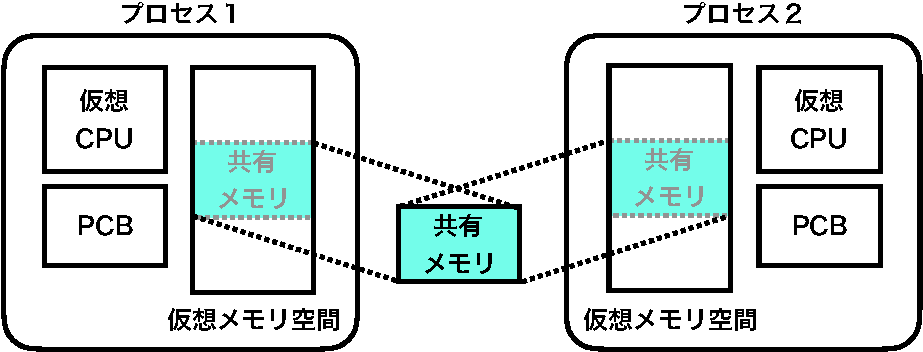
\includegraphics[scale=0.6]{Fig/ipcShearedMemory-crop.pdf}
  \end{center}
  \begin{itemize}
  \item 同じ物理メモリを複数のプロセスの仮想メモリ空間に貼り付ける.
  \item MMU(Memory Management Unit)の働きで可能になる.
  \item 貼り付けが終わればシステムコールなしでデータ交換可能.
  \item プロセス間の同期機構は他に必要.
  \end{itemize}
\end{frame}

\begin{frame}
  \frametitle{UNIXの共有メモリサーバ例(前半)}
  \lstinputlisting{Lst/ipcUnixShearedMemoryServer1.c}
\end{frame}

\begin{frame}
  \frametitle{UNIXの共有メモリサーバ例(後半)}
  \lstinputlisting{Lst/ipcUnixShearedMemoryServer2.c}
\end{frame}

\begin{frame}
  \frametitle{UNIXの共有メモリクライアント例(前半)}
  \lstinputlisting{Lst/ipcUnixShearedMemoryClient1.c}
\end{frame}

\begin{frame}
  \frametitle{UNIXの共有メモリクライアント例(後半)}
  \lstinputlisting{Lst/ipcUnixShearedMemoryClient2.c}
\end{frame}

\begin{frame}
  \frametitle{UNIXの共有メモリプログラム実行例}
  \lstinputlisting{Lst/ipcUnixShearedMemoryTest.txt}
  \begin{itemize}
  \item このプログラムは相互排除をやっていない.
  \item このプログラムは{\bf 使用してはならない}.
  \end{itemize}
\end{frame}

\section{メッセージ通信}
\begin{frame}
  \frametitle{メッセージ通信}
  \begin{center}
    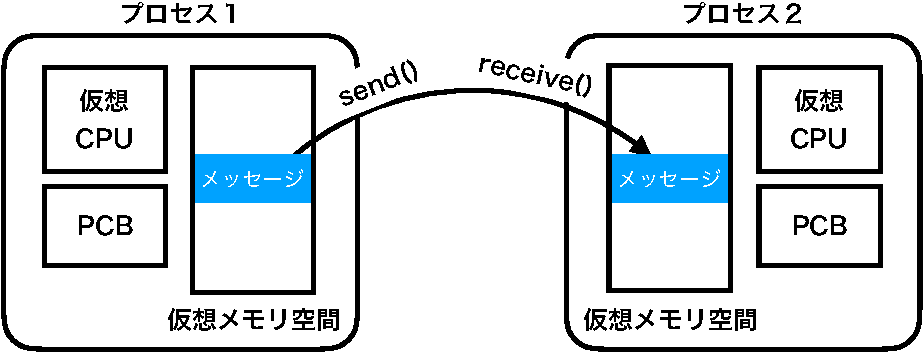
\includegraphics[scale=0.6]{Fig/ipcMessagePassing-crop.pdf}
  \end{center}
  \begin{itemize}
  \item {\tt send()}システムコールでメッセージを送信する.
  \item {\tt receive()}システムコールでメッセージを受信する.
  \item メッセージ通信は同期機構も含んでいる.
  \end{itemize}
\end{frame}

\begin{frame}
  \frametitle{通信相手の指定方式(Naming)}
  \begin{center}
    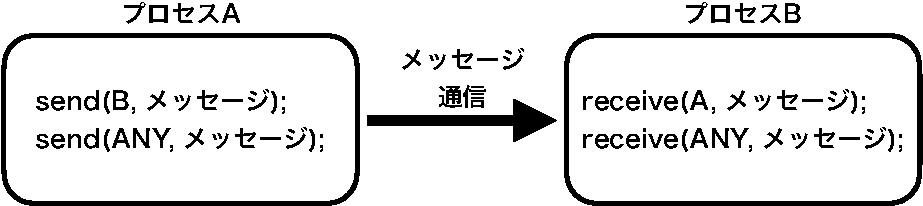
\includegraphics[scale=0.6]{Fig/ipcDirect-crop.pdf}\\
    直接指定方式
    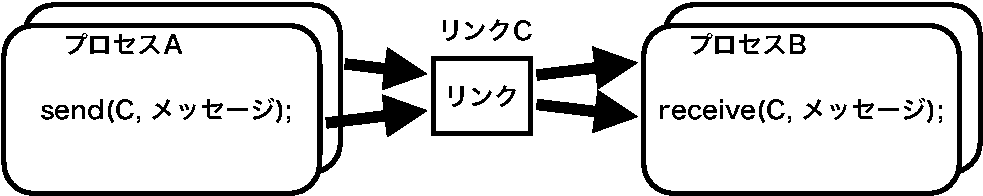
\includegraphics[scale=0.6]{Fig/ipcIndirect-crop.pdf}\\
    間接指定方式
  \end{center}
  \begin{itemize}
  \item 直接指定方式でもANYを用いることで多対多通信が可能.
  \item 間接指定方式は自然に多対多通信が可能
  \end{itemize}
\end{frame}

\begin{frame}
  \frametitle{通信方式}
  一般に
  \begin{itemize}
  \item バッファリング(あり/なし)
  \item メッセージ長(固定/可変)
  \item メッセージ形式(タグあり/なし)
  \item 同期方式
    \begin{itemize}
    \item 非同期方式(ノンブロッキング)
    \item 同期方式(ブロッキング)
    \item ランデブー方式
    \end{itemize}
  \end{itemize}

  UNIXの場合は
  \begin{itemize}
  \item 間接指定方式
  \item バッファリング=あり
  \item メッセージ長=可変長
  \item メッセージ形式=タグあり
  \item 同期方式/非同期方式どちらも可能
  \end{itemize}
\end{frame}

\begin{frame}
  \frametitle{UNIXのメッセージ通信プログラム例1}
  \lstinputlisting{Lst/ipcUnixMessage.h}
  \lstinputlisting{Lst/ipcUnixMessageWriter1.c}
\end{frame}

\begin{frame}
  \frametitle{UNIXのメッセージ通信プログラム例2}
  \lstinputlisting{Lst/ipcUnixMessageWriter2.c}
\end{frame}

\begin{frame}
  \frametitle{UNIXのメッセージ通信プログラム例3}
  \lstinputlisting{Lst/ipcUnixMessageReader1.c}
\end{frame}

\begin{frame}
  \frametitle{UNIXのメッセージ通信プログラム例4}
  \lstinputlisting{Lst/ipcUnixMessageReader2.c}
  \lstinputlisting{Lst/ipcUnixMessageTest.txt}
\end{frame}

\section{TacOSのメッセージ通信機構}
\begin{frame}
  \frametitle{TacOSのメッセージ通信機構}
  クライアント・サーバモデルに特化したプロセス間通信機構を提供する.
  \begin{center}
    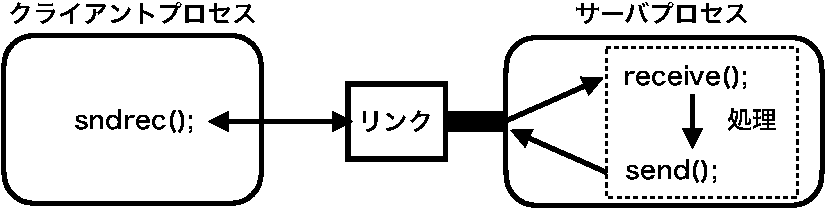
\includegraphics[scale=0.6]{Fig/tacosMessage-crop.pdf}
  \end{center}
  \begin{enumerate}
  \item サーバプロセスが{\bf リンク}を所有し通信を待ち受ける.
  \item クライアントプロセスは{\tt sndrec()}関数でメッセージを送信する.
  \item サーバプロセスは{\tt receive()}関数を用いてメッセージを受信する.
  \item サーバプロセスはメッセージの内容に合った処理を行う.
  \item サーバプロセスは処理結果を{\tt send()}関数を用いて返信する.
  \item {\tt sndrec()}関数が完了しクライアントは処理結果を受取る.
  \end{enumerate}
\end{frame}

\begin{frame}
  \frametitle{TacOSのリンク構造体}
  \lstinputlisting{Lst/tacosLink.hmm}
  \begin{itemize}
  \item リンクはサーバが所有する.
  \item セマフォを用いて相互排除と同期を行う.
  \item リンクに書き込めるメッセージの形式は固定.
  \end{itemize}
\end{frame}

\begin{frame}
  \frametitle{TacOSのリンク作成ルーチン}
  \lstinputlisting{Lst/tacosNewLink.cmm}
  \begin{itemize}
  \item 割込み禁止による相互排除を行っている.
  \item リンクの廃棄(削除)はできない.
  \item セマフォを三つ割当てる.
  \end{itemize}
\end{frame}

\begin{frame}
  \frametitle{TacOSのメッセージ通信ルーチン(サーバ用)}
  \lstinputlisting{Lst/tacosSendReceive.cmm}
  \begin{itemize}
  \item {\tt receive()}はリンクにメッセージが届くのを待つ.
  \item {\tt receive()}はメッセージが書き込まれたリンクを返す.
  \item {\tt send()}はリンクに処理結果(16bit)を返信する.
  \end{itemize}
\end{frame}

\begin{frame}
  \frametitle{TacOSのメッセージ通信使用例(サーバ側)}
  \lstinputlisting{Lst/tacosPmMain.cmm}
  \begin{itemize}
  \item プロセスマネージャ(サーバプロセス)の例.
  \item サーバはリンクを作成した後,受信,処理,返信を繰り返す.
  \item {\tt receive()}を用いてリンクからメッセージを受信.
  \item {\tt pmSysCall()}がプロセスマネージャの処理ルーチン.
  \item {\tt send()}を用いてクライアントに処理結果を返す.
  \end{itemize}
\end{frame}

\begin{frame}
  \frametitle{TacOSのメッセージ通信ルーチン(クライアント用)}
  \lstinputlisting{Lst/tacosSndRec.cmm}
  \begin{itemize}
  \item {\tt iSemv()}を使用するので割込み禁止による相互排除が必要.
  \item クライアント間での相互排除にセマフォ{\tt s2}を使用.
  \end{itemize}
\end{frame}

\begin{frame}
  \frametitle{TacOSのメッセージ通信使用例(クライアント側)}
  \lstinputlisting{Lst/tacosPmExec.cmm}
  \begin{itemize}
  \item execシステムコールを例にする.
  \item execは{\tt path}のプログラムを新しいプロセスで実行する.
  \item 上のプログラムはSVC割込みハンドラから呼出される.
  \item SVC割込みハンドラはシステムコールの種類を判断し,
    execシステムコールの場合に上のルーチンを呼出す.
  \item 割込みハンドラはプロセスのコンテキストで実行される.
  \item execシステムコールはプロセスマネージャが処理する.
  \item プロセスマネージャへのメッセージ通信により処理を依頼する.
  \item {\tt \_AtoI()}関数は参照(アドレス)を{\tt int}型に変換する.
  \end{itemize}
\end{frame}

\begin{frame}
  \frametitle{TaC7とTaC(参考)}
  \begin{minipage}{0.58\columnwidth}
    \begin{center}
      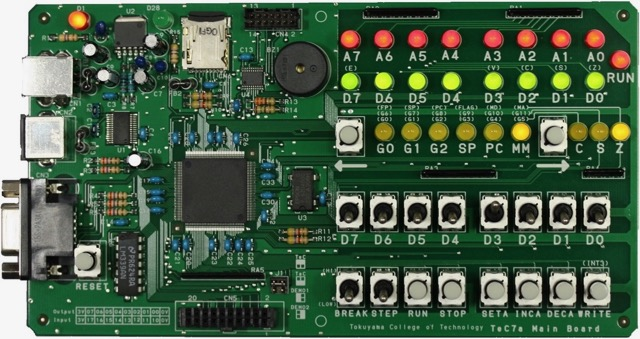
\includegraphics[scale=0.27]{Photo/TeC7.jpg}\\
      (a) TeC7の写真
    \end{center}
  \end{minipage}
  \begin{minipage}{0.38\columnwidth}
    \begin{center}
      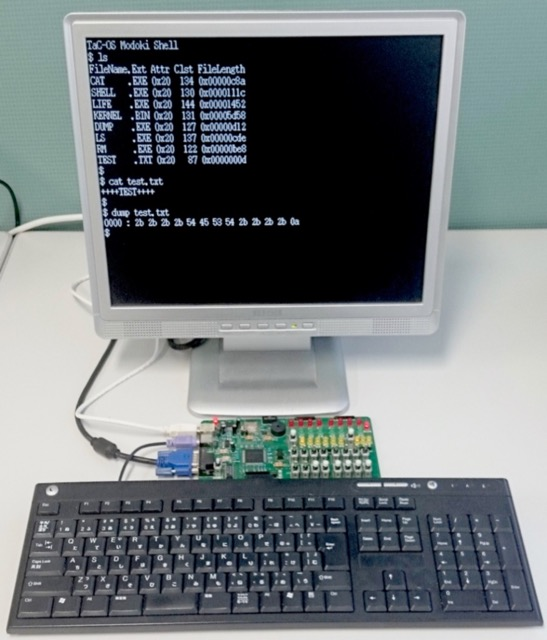
\includegraphics[scale=0.22]{Photo/TaC.jpg}\\
      (b) TaCとしての使用例
    \end{center}
  \end{minipage}
\vfill
TeC7は,TacOSを書き込んだマイクロSDカードを装着すると,
簡単なPC(TaC)として使用できる.
\end{frame}

\begin{frame}
  \frametitle{TaCのハードウェア(参考)}
  \fig{scale=0.49}{tacBlock-crop.pdf}
\end{frame}

\begin{frame}
  \frametitle{一般的なPCのハードウェア(参考)}
  \fig{scale=0.40}{hardBlock-crop.pdf}
\end{frame}

\begin{frame}
  \frametitle{TacOSの構造(参考)}
  \fig{scale=0.49}{tacosOrganization-crop.pdf}
\end{frame}

\begin{frame}
  \frametitle{マイクロカーネル方式(参考)}
  \fig{scale=0.49}{microkernel-crop.pdf}
\end{frame}

\begin{frame}
  \frametitle{オペレーティングシステムの構造(参考)}
  \fig{scale=0.49}{osOrganization-crop.pdf}
\end{frame}
\end{document}
